\section*{Ejercicios de tipo test}
\addcontentsline{toc}{section}{Ejercicios de tipo test}


\begin{ejercicio}¿Qué sale cuando ejecutamos el siguiente código?

\begin{python}
x = True
y = False
z = False
if not x or y:
    print(1)
elif not x or not y and z:
    print(2)
elif not x or y or not y and x:
    print(3)
else:
    print(4)
\end{python}


\begin{choices}
    \choice 1
    \choice 2
    \choice 3 %CORRECT
    \choice 4
\end{choices} 
\end{ejercicio}

%\solucion{C}


\begin{ejercicio}¿Qué es el resultado de la expresión: \verb|3*1**3|?

\begin{choices}
    \choice 3 %CORRECT
    \choice 9
    \choice 1
    \choice 27
\end{choices} \end{ejercicio}
%\solucion{A}

\begin{ejercicio}¿Qué sale cuando ejecutamos el siguiente código?

\begin{python}
if (5>10):
    print("examen")
elif 8!=9:
    print("lunes")
else:
    print(11 de noviembre)
\end{python}

\begin{choices}
    \choice examen
    \choice lunes %CORRECT
    \choice 11 de noviembre
    \choice syntax error
\end{choices} \end{ejercicio}

%\solucion{B lunes}


\begin{ejercicio}Imagine las siguientes instrucciones en Python:
\begin{python}
x = True
y = False
z = False

if x or y and z:
    print("yes")
else:
    print("no")
\end{python}

¿Cual es el resultado?

\begin{choices}
    \choice yes %CORRECT
    \choice no
    \choice Excepción
    \choice Error de sintaxis
\end{choices} \end{ejercicio}

\begin{ejercicio}Imagine las siguientes instrucciones en Python:
\begin{python}
if (9 < 0) and (0 < -9):
    print("hello")
elif (9 > 0) or False:
    print("good")
else:
    print("bad")
\end{python}

¿Cual es el resultado?

\begin{choices}
    \choice error
    \choice hello
    \choice good %CORRECT
    \choice bad
\end{choices} \end{ejercicio}


\begin{ejercicio}¿Cuál de las siguientes expresiones booleanas NO es equivalente a las otras?

\begin{choices}
    \choice \pythoninline{not(-6>10 or -6==10)} %CORRECT
    \choice  \pythoninline{not(-6<0 or -6>10)}
    \choice \pythoninline{-6>=0 and -6<=10}
    \choice \pythoninline{not(-6<10 or -6==10)}
\end{choices} \end{ejercicio}


\begin{ejercicio}
¿Qué imprime por pantalla el siguiente programa?

\begin{python}
a = True
b = False
c = False

if b or c and a or b:
    print("no")
else:
    print("yes")
    \end{python}

\begin{choices}
    \choice no
    \choice yes %CORRECT
    \choice Excepción
    \choice Error de sintaxis
\end{choices} 
\end{ejercicio}


\begin{ejercicio} ¿Qué imprime por pantalla el siguiente programa?
\begin{python}
if ("irajo" < "iraka"):
    print(1, end=" ")
if ("erribas" < "erriba"):
    print(2, end=" ")
if ("orribo" < "irribu"):
    print(3, end=" ")
if ("oribas" < "oribat"):
    print(4, end=" ")
if ("MARCA" < "YRBA"):
    print(5, end=" ")    
if ("vribo" < "vrriba"):
    print(6, end=" ")
\end{python}

\begin{choices}
    \choice 1 3 4 5 6
    \choice 1 4 6
    \choice 1 4 5 6   %CORRECT
    \choice 1 2 5 6
\end{choices}
\end{ejercicio}

\newpage

\begin{ejercicio} Considera las siguientes instrucciones en Python:


\begin{python}
cond = math.sqrt(a ** 5 - b)
if (cond >= 0):
    b = 9
\end{python}

\pythoninline{a}  es \fbox{1}

\pythoninline{math.sqrt(a ** 5 - b)}  es \fbox{2}

\pythoninline{x >= 0} es  \fbox{3}

\begin{choices}
    \choice \fbox{1} = un operando, \fbox{2} = una expresión y \fbox{3} = una condición   %CORRECT
    \choice \fbox{1} = un operador, \fbox{2} = una instrucción y \fbox{3} = un booleano
    \choice \fbox{1} = una instrucción, \fbox{2} = una expresión y \fbox{3} = una ecuación 
    \choice \fbox{1} = un operando, \fbox{2} = una ecuación y \fbox{3} = una expresión
\end{choices}
\end{ejercicio}


\begin{ejercicio} Imagina que tenemos el siguiente programa:

\begin{python}
try:
    x = int(input("Please enter a number: "))
    print(50/x)
except ValueError:
    print('That is not good, closing...')
except:
    print("Something else went wrong, closing...")
\end{python}

Ejecutamos el programa 3 veces:

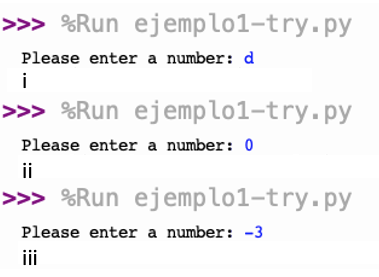
\includegraphics[width=0.4\textwidth]{book/Spanish/04_Bucles/images/exception-fig.png}

¿Cuál será la salida en cada caso (representado por i, ii, e iii)?

\begin{choices}
    \choice    %CORRECT
    i =   That is not good, closing...\\ 
    ii =  Something else went wrong, closing...\\ 
    iii =  -16.666666666666668
    \choice 
    i =   Something else went wrong, closing...\\ 
    ii = That is not good, closing...\\ 
    iii =  -16.666666666666668
   \choice 
     i =  That is not good, closing...\\ 
    ii =  That is not good, closing...\\ 
    iii =  Something else went wrong, closing...
    
    \choice 
     i =  0.5\\ 
    ii =  Something else went wrong, closing...\\ 
    iii =  -16.666666666666668   
\end{choices}
\end{ejercicio}

